\documentclass[paper=a4, fontsize=11pt]{scrartcl}
\usepackage{enumerate}
\usepackage{amsmath}
\usepackage{amssymb}
\usepackage{tikz}
\newcommand{\parens}[1]{ \left( #1 \right) }
\begin{document}
\noindent Willy Xiao and Kevin Eskici \\ STAT 221 \\Pset 4\\ Nov 4, 2014
\begin{enumerate}[\text{question }1.]
  \item
    \begin{enumerate}[1]
      
      \item   
      $p(\lambda, \theta) \propto \lambda^{-1}$\\
      $\begin{bmatrix} N \\ \theta \end{bmatrix} = f\parens{\begin{bmatrix} \lambda \\ \theta \end{bmatrix}}$\\
      $p(N, \theta) = p(\lambda, \theta) * \begin{Vmatrix}  \frac{\partial \lambda}{\partial N} &  \frac{\partial \theta}{\partial N} \\ \frac{\partial \lambda}{\partial \theta} &  \frac{\partial \theta}{\partial \theta} \end{Vmatrix}$\\
      Our Jacobian is $\begin{vmatrix} \theta & {-\lambda N^{-2}} \\N & 1 \end{vmatrix}$\\
      and its determinant is $\theta + \frac{\lambda}{N}$\\\\
      $p(N, \theta) \propto \frac{1}{\theta N} * (\theta + \frac{\lambda}{N})$\\
      $= \frac{1}{\theta N} * (\theta + \frac{\theta N}{N})$\\
      $= \frac{2}{N}$\\
      $\propto \frac{1}{N}$
      \\This prior favors smaller values of N.

      \item It is an improper prior: $\int_0^\infty{\int_0^1{\lambda^{-1}}}d\theta d\lambda \rightarrow \ln(\infty) - \ln(0)$. This cannot integrate to 1 with any constant factor.
	
	\item No $p(\lambda, \theta)$ is not a non-informative prior in the sense of Jeffreys.\\ 
	$p(y_i| \theta, \mu) = \frac{(\theta \mu)^{y_{i}}}{y_{i}!} e^{-\theta \mu}$\\
	$y_i log(\theta | \mu ) - log({y_i}!) - \frac{\theta}{\mu}$\\
	$\frac{\partial I}{\partial \theta} = y_i (\theta \mu)^{-1} \mu - \frac{1}{\mu} = 
	y_i (\theta)^{-1} - \frac{1}{\mu}$\\
	$\frac{\partial I}{\partial \mu} = y_i \mu + \theta \mu^{-2}$	\\
	$\frac{\partial^2 I}{\partial \theta^2} = -{y_i}\theta^{-2}$\\
	$\frac{\partial^2 I}{\partial \mu^2} = y_i - 2\theta \mu^{-3}$\\
	$\frac{\partial^2 I}{\partial \mu \partial \theta} = \mu^{-2}$\\
	$\frac{\partial^2 I}{\partial \theta \partial \mu } = \mu^{-2}$\\
	This gives us the fisher's information matrix $\begin{pmatrix}-{y_i}\theta^{-2} & \mu^{-2} \\\mu^{-2} & y_i - 2\theta \mu^{-3} \end{pmatrix}$, which has determinant $({y_i}\theta^{-2})^2 - 2\theta \mu^{-3}y_i - \mu^{-4}$, the square root of which is not proportional to $\frac{(\theta \mu)^{y_{i}}}{y_{i}!} e^{-\theta \mu}$.


	
	\item See R code and MCMC design note. Also figures 1 and 2 show posterior contours for an impala and waterbuck chain (2 were chosen arbitrarily, but they all look similar). Figures 3 and 4 are additional diagnostic plots for one of the impala chains-autocorrelation and mixing look good. To run diagnostics on other chains, just load the corresponding chain in $checkdiagnostics.R$ and run the script (note the R datafiles for chains are not included due to space constraints but will be generated when you run the slurm job).
	
	\item Posterior for N\\
	$\int^1_0 \parens{\prod_{i=1}^n\binom{N}{x_i}\theta^{x_i}(1-\theta)^{N - x_i}}* \frac{1}{N} d\theta$\\
	$=\int^1_0 \parens{\prod_{i=1}^n\binom{N}{x_i}}\theta^{\Sigma x_i}(1-\theta)^{nN - \Sigma x_i}* \frac{1}{N} d\theta$\\
	$= \frac{1}{N} \int^1_0 \theta^{\Sigma x_i}(1-\theta)^{nN - \Sigma x_i}\prod_{i=1}^n\binom{N}{x_i} d\theta$\\
	$= \frac{1}{N} \prod_{i=1}^n\binom{N}{x_i}  \int^1_0 \theta^{\Sigma x_i}(1-\theta)^{nN - \Sigma x_i}d\theta$\\
	If we define $S = \Sigma x_i$, the integral above has the form of a\\ 
	Beta($\alpha=S+1, \beta=nN - S + 1$ ) pdf\\
	Using this we get, $\frac{(nN-S)!}{(nN + 1)!N)}$, which when $n=1$, $\rightarrow \frac{x_i}{N(N+1)}$\\\\
	Using our function $find.norm.log.const$ defined in $keskici\_wxiao\_ps4\_post.R$, we found that the normalizing constant for the impala dataset was $e^{15.63617}$ and the normalizing constant for the waterbuck dataset was $e^{16.83744}$. Figures 5 and 6 show the posteriors for Impala and Waterbuck respectively.
	
	% \item Give POSTERIOR PROBS N $>$ 100
  \item predicted $p(N > 100)$ \\
    \begin{center}
      \begin{tabular}{ l | c || r }
        chain & impala & waterbuck \\
        \hline
        analytic & 0.3401253 & 0.9576785 \\ \hline
        1 & 0.3283853 & 0.9572161 \\
        2 & 0.3261333 & 0.9576201 \\
        3 & 0.3268553 & 0.9574501 \\
        4 & 0.3289333 & 0.9575941 \\
        5 & 0.3274193 & 0.9578081 \\
        6 & 0.3266493 & 0.9574521 \\
        7 & 0.3288193 & 0.9577741 \\
        8 & 0.3258933 & 0.9573301 \\
        9 & 0.3313833 & 0.9573721 \\
        10 & 0.3273273 & 0.9572281 \\ \hline
        mean & 0.3277799 & 0.9574845 \\
        std. & 0.001649921 & 0.000209621
      \end{tabular}
    \end{center}

    \end{enumerate}
    Our mcmc chains for both impala and waterbuck appear to be pretty good for predicting $p(N > 100)$ relative to each other (ie very small standard deviation between each chain). The analytic probability for the waterbuck dataset is close to the mean of the waterbuck posteriors, but the analytic probability of the impala dataset is further off. The source of error for the impala dataset, might come from numerically computing the normalizing constant which also comes from the numerical dataset.

    Note about MCMC Design: We ran a MCMC Metroplis-Hastings algorithm. We tried many different proposal methods such as generating a $(N, \theta)$ from a multivariate normal, or generating $N$ from a binomial. Ultimately we found the best design to be generating a $\lambda = N*\theta$ from a normal distribution centered at $N_{t-1}*\theta_{t-1}$ and then generating a $\theta$ from a uniform. This allows us to preserve the symmetry of $J(\theta | \theta_{t-1}) = J( \theta_{t-1} | \theta)$.
\end{enumerate}

\clearpage
Appendix: \\
\begin{figure}[h!]
  \caption{Countour plot for 8th Impala Chain}
  \centering
	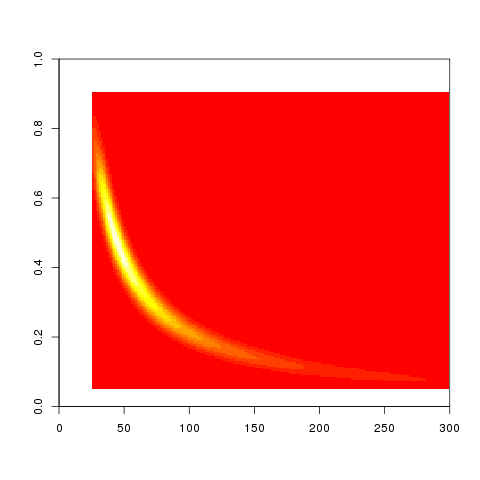
\includegraphics[scale=.8]{keskici_wxiao_ps4_task_impala_run5_plot8.png}
\end{figure}

\begin{figure}[h!]
  \caption{Countour plot for 5th Waterbuck Chain}
  \centering
	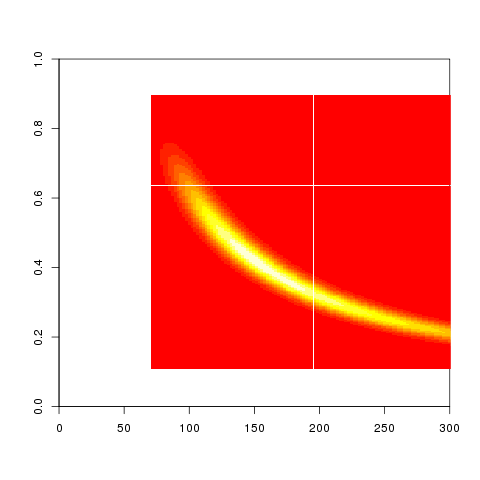
\includegraphics[scale=.8]{keskici_wxiao_ps4_task_waterbuck_run5_plot5.png}
\end{figure}

\begin{figure}[h!]
  \caption{Trace plots for 8th Impala Chain}
  \centering
	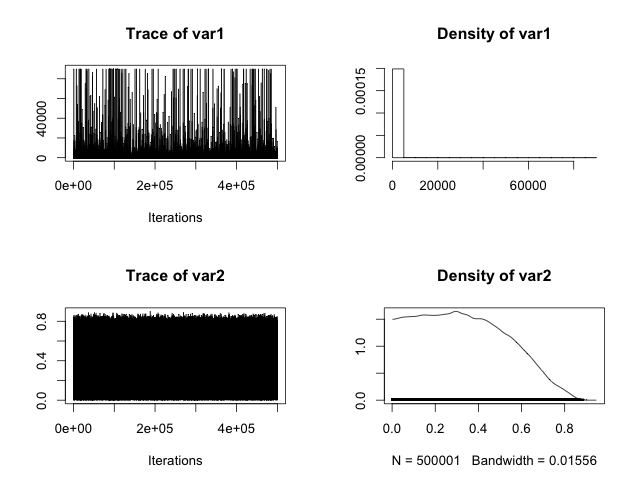
\includegraphics[scale=.8]{Rplot_job8a.png}
\end{figure}

\begin{figure}[h!]
  \caption{Autocorrelation plot for 8th Impala Chain}
  \centering
	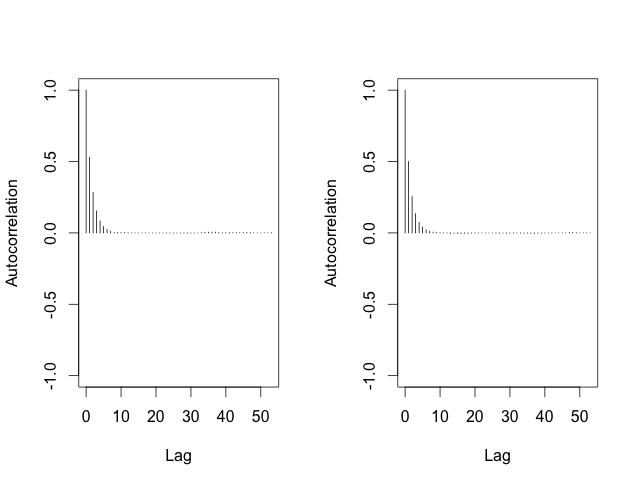
\includegraphics[scale=.8]{Rplot_job8b.png}
\end{figure}

\begin{figure}[h!]
  \caption{Posterior for Impala Dataset}
  \centering
	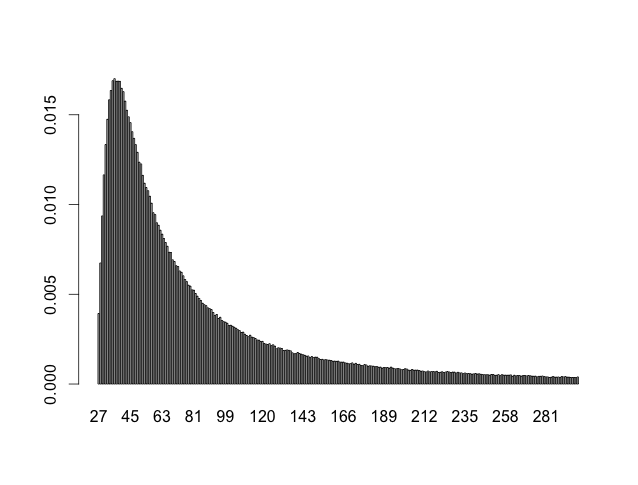
\includegraphics[scale=.8]{impala.png}
\end{figure}

\begin{figure}[h!]
  \caption{Posterior for Waterbuck Dataset}
  \centering
	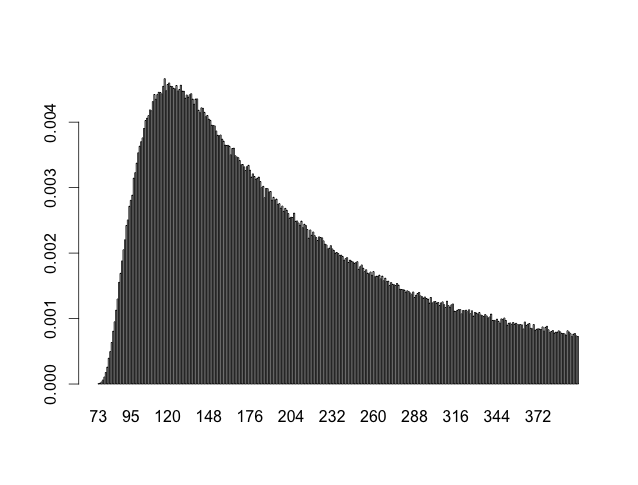
\includegraphics[scale=.8]{waterbuck.png}
\end{figure}

\end{document}
